\chapter{Практические задания}
\section{Задание}
\vspace{-0.7cm}
Используя хвостовую рекурсию, разработать программу, позволяющую найти:
\vspace{-0.5cm}
\begin{enumerate}
	\item n!;
	\item n-е число Фибоначчи.
\end{enumerate}
\vspace{-0.5cm}
Убедиться в правильности результатов.
Для одного из вариантов ВОПРОСА и каждого задания составить таблицу,
отражающую конкретный порядок работы системы.

Код программы представлен на листинге \ref{lst:code}.
\begin{lstlisting}[label=lst:code, basicstyle=\footnotesize, caption=Код программы]
predicates
	factorial(integer, integer).
	factorial(integer, integer, integer).
	
	fib(integer, integer).
	fib(integer, integer, integer, integer).
clauses
	factorial(N, Factorial_N, Factorial_M) :-  N > 1,
									  Temp_factorial_N = Factorial_M * N,
									  M = N - 1, !,
								factorial(M, Factorial_N, Temp_factorial_N).
	factorial(_, Factorial_M, Factorial_M).
	factorial(N, Factorial_N) :- factorial(N, Factorial_N, 1).
	
	fib(N, Fib_N, Last_N, Last_fib) :- N > 3, 
									   Temp_fib = Last_N + Last_fib, 
									   Temp_N = N - 1, !,
									   fib(Temp_N, Fib_N, Last_fib, Temp_fib).
	fib(_, Temp_fib, _, Temp_fib).
	fib(1, 0).
	fib(N, Fib_N) :- fib(N, Fib_N, 1, 1).
goal
	%factorial(5, Factorial_N).
	fib(4, Fib_elem).
\end{lstlisting}

Ниже на рисунках \ref{image:table_1} \ref{image:table_2} приведена таблица порядка поиска ответа для нахождение факториала:
\begin{figure}[H]
	\centering{
		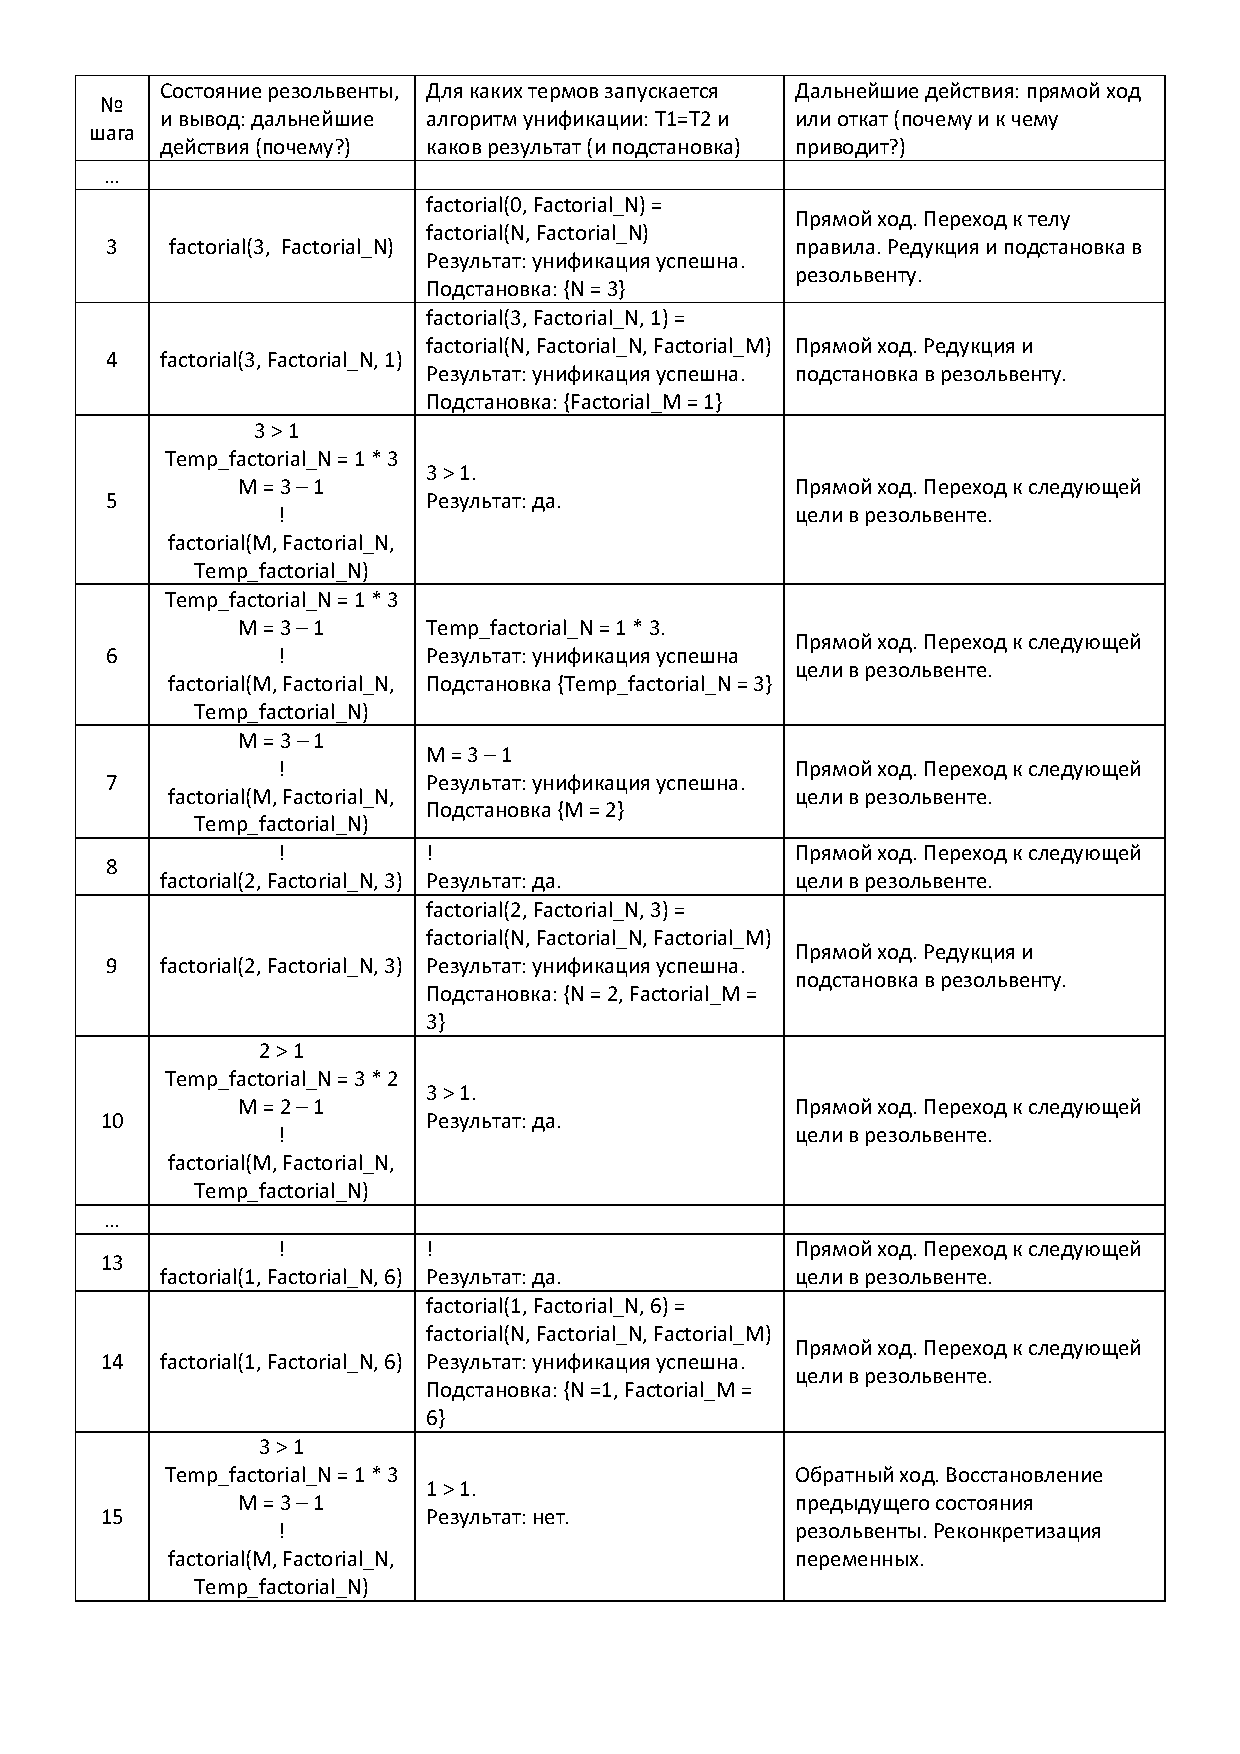
\includegraphics[scale=0.9]{images/table_6_1.pdf}
		\caption{Таблица порядка поиска ответов для нахождение факториала.}
		\label{image:table_1}
	}
\end{figure}

\begin{figure}[H]
	\centering{
		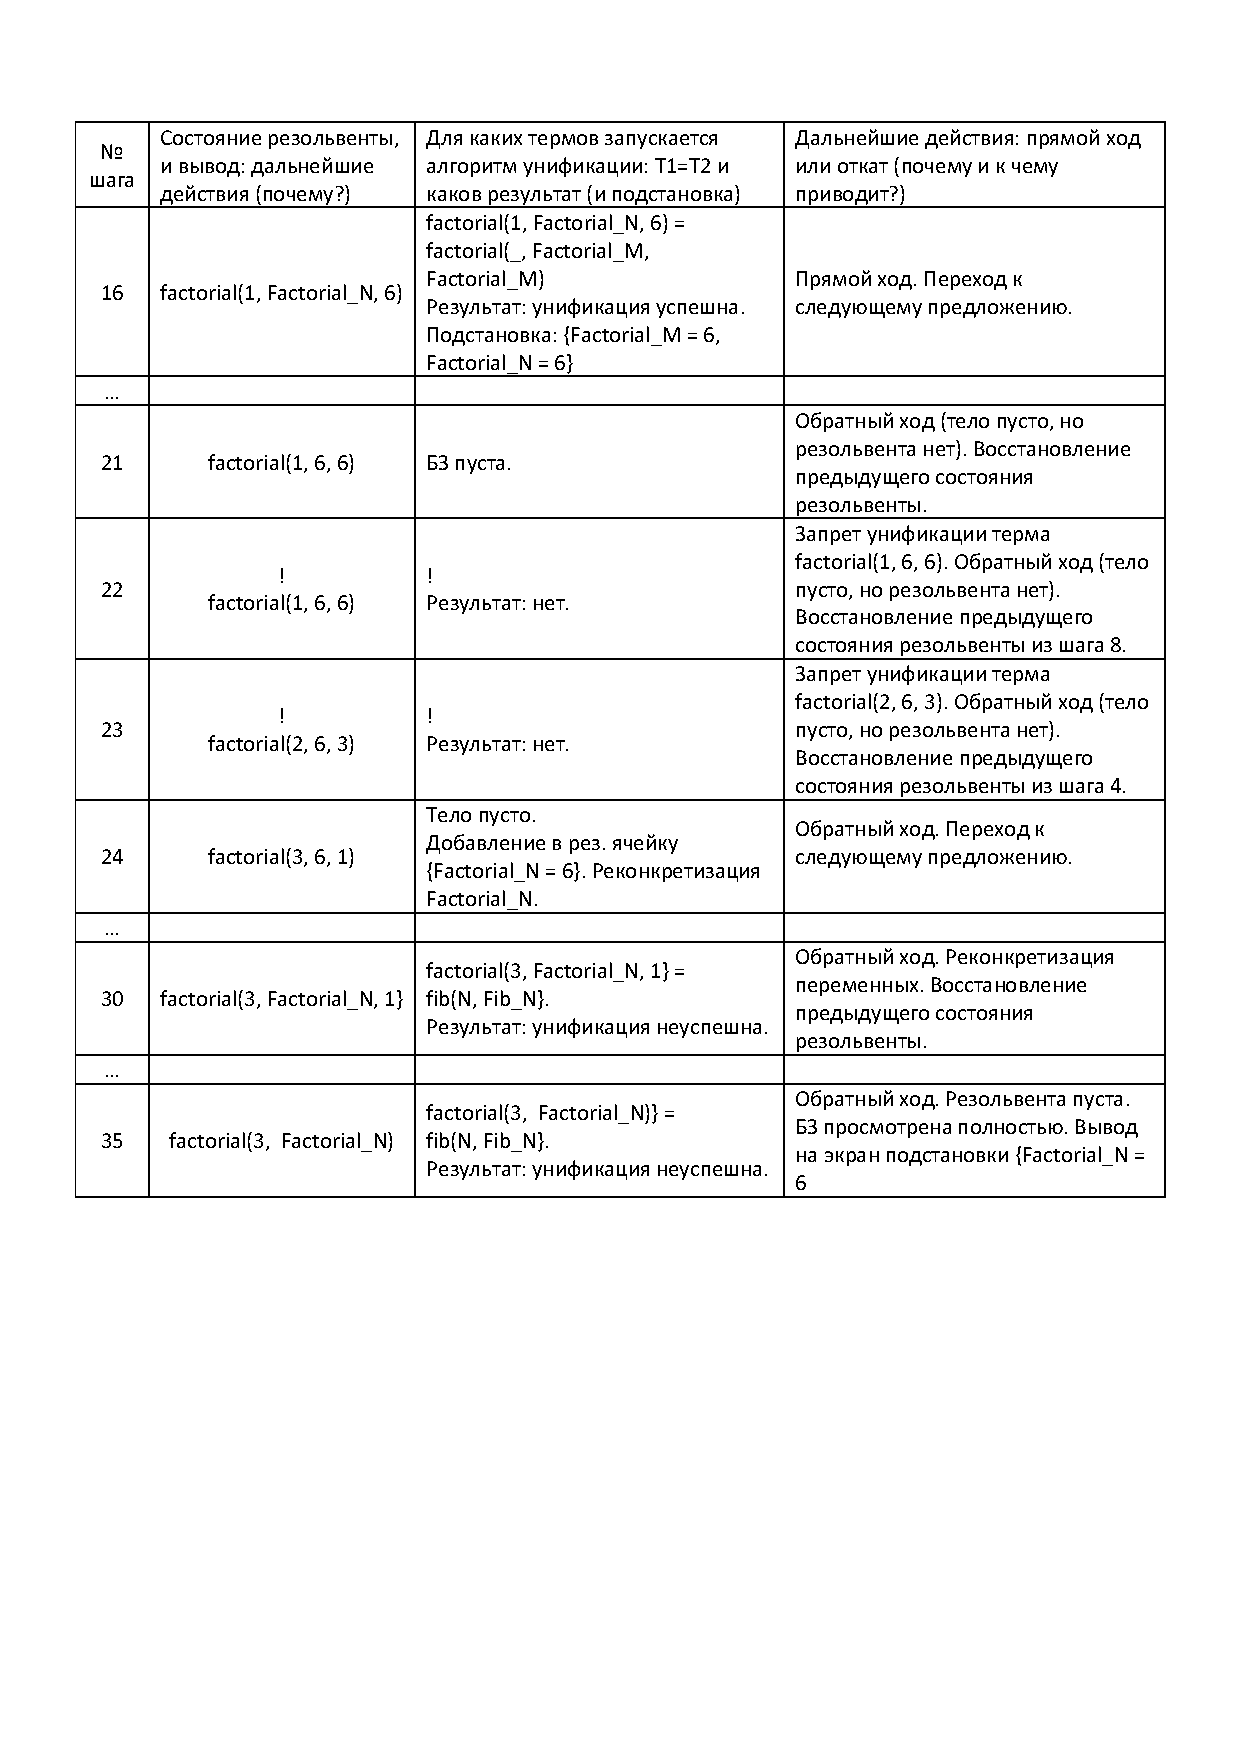
\includegraphics[scale=0.9]{images/table_6_2.pdf}
		\caption{Таблица порядка поиска ответов для нахождение факториала (продолжение).}
		\label{image:table_2}
	}
\end{figure}

Ниже на рисунке \ref{image:table_3} и \ref{image:table_4} приведена таблица порядка поиска ответа для нахождения значения N-ого числа Фибоначчи:
\begin{figure}[H]
	\centering{
		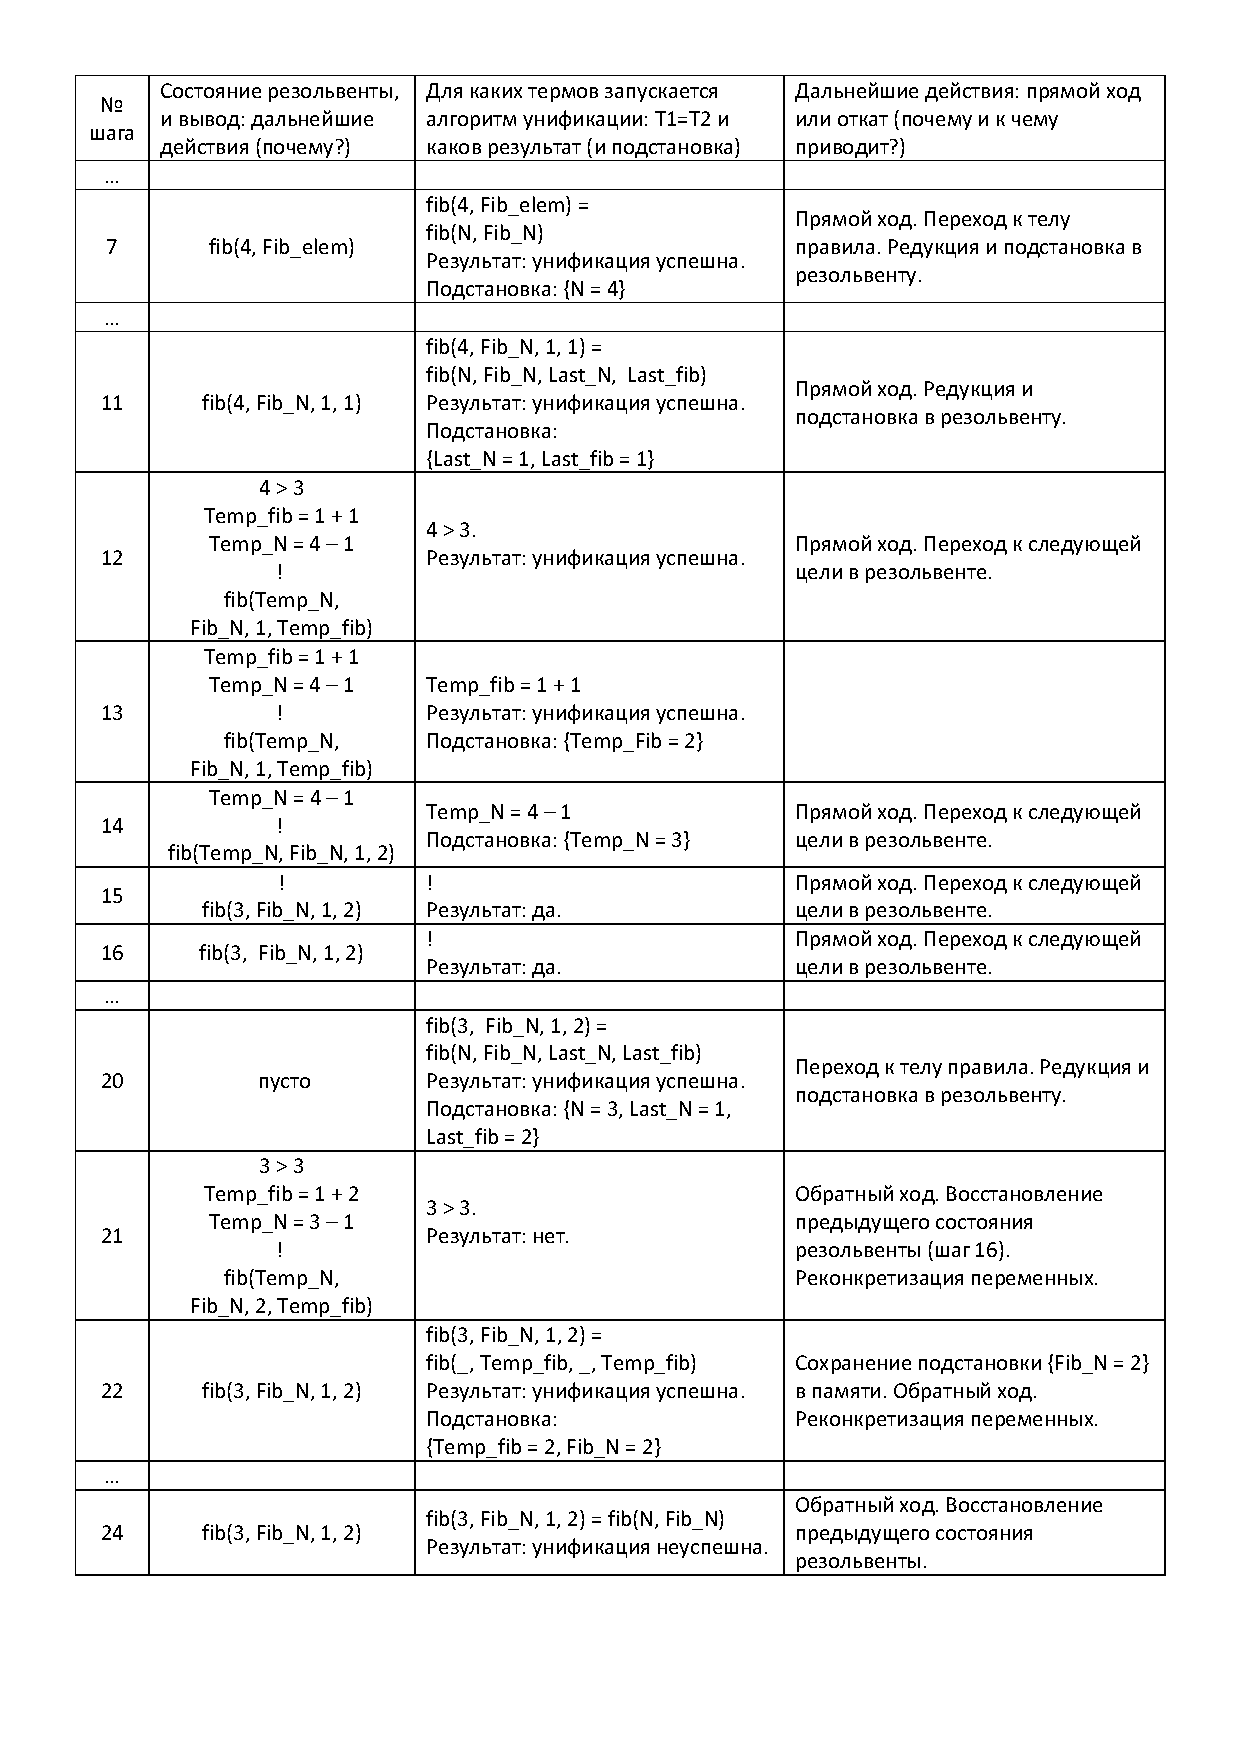
\includegraphics[scale=0.9]{images/table_6_3.pdf}
		\caption{Таблица порядка поиска ответов для нахождения значения N-ого числа Фибоначчи.}
		\label{image:table_3}
	}
\end{figure}

\begin{figure}[H]
	\centering{
		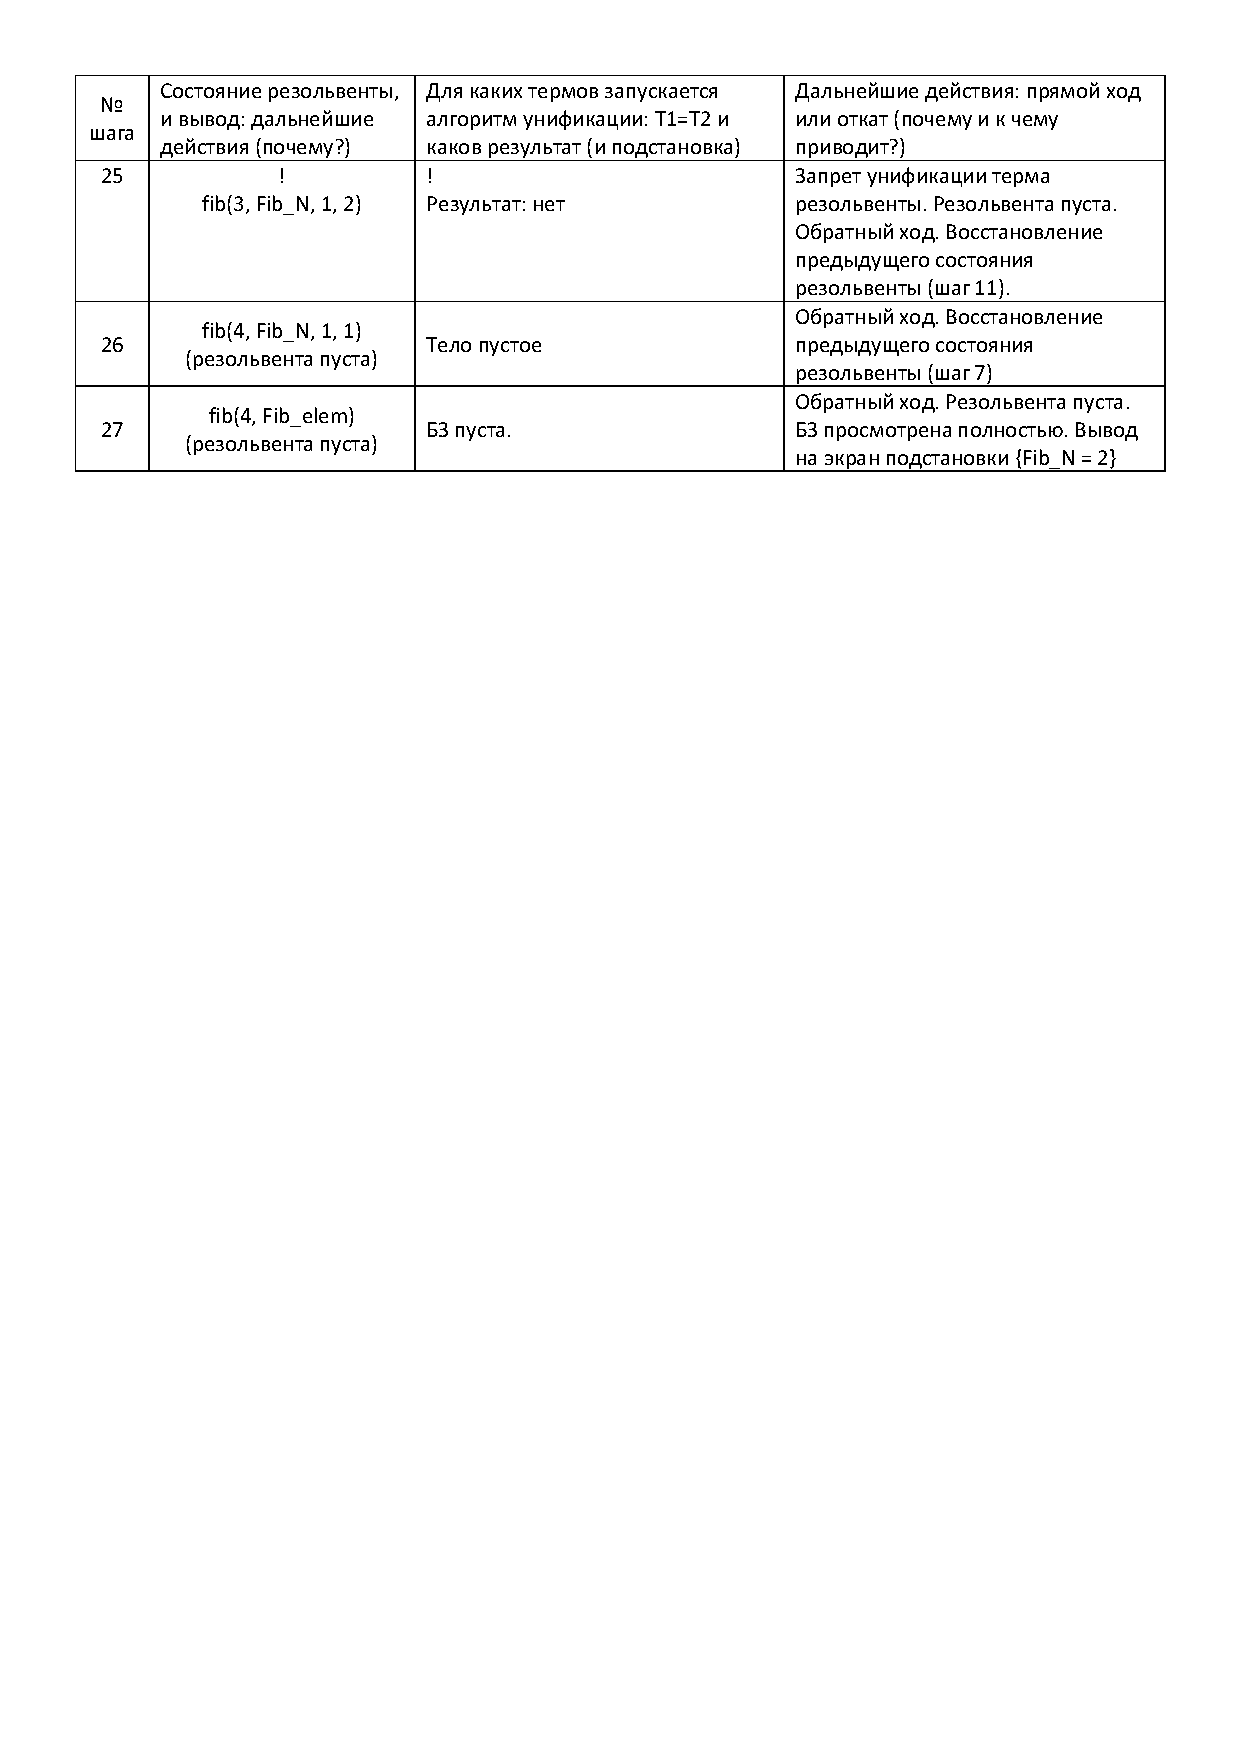
\includegraphics[scale=0.9]{images/table_6_4.pdf}
		\caption{Таблица порядка поиска ответов для нахождения значения N-ого числа Фибоначчи (продолжение).}
		\label{image:table_4}
	}
\end{figure}